%\documentclass[pdf]{prosper}
% for printing
%\documentclass[ps2pdf]{prosper}
% for using Acrobat Distiller
\documentclass[pdf,distiller]{prosper}

% Introduction to the `HA-Prosper' package.
% Created by: Hendri Adriaens
%             http://center.uvt.nl/phd_stud/adriaens
%             Center for Economic Research
%             Tilburg University, the Netherlands

%================================================
% Please also read the manual of HA-prosper and
% of the specific style you are using since some
% features of this example might not be supported
% by the style you use.
%================================================

\usepackage[toc,hlsections,highlight,Cornell]{HA-prosper}

\HAPsetup{%
trans=Wipe,
tsnav=FullScreen,
nsnav=ShowBookmarks,
lf={\href{mailto:lars.vilhuber@cornell.edu}{Lars Vilhuber}, John Abowd and
  Bryce Stephens},
rf={\today},
iacolor=gray,
stype=1
}

%\renewcommand{\theequation}{}
%\usepackage{newcent}
%\usepackage{helvet}
%\usepackage{helvetic}
%\usepackage{ncntrsbk}
%\usepackage{bookman}
%\usepackage{avantgar}
%\usepackage{helvet}

% etc. 
\newcommand{\mytitle}{The LEHD Infrastructure Files}
\newcommand{\mysubtitle}{and the Creation of the Quarterly Workforce Indicators} 
\newcommand{\myshorttitle}{LEHD/ QWI Overview }
\newcommand{\myauthors}{John M. Abowd{\footnotesize
    $^{\spadesuit,\clubsuit}$},
 Bryce  E. Stephens{\footnotesize$^\clubsuit$} and 
 Lars Vilhuber{\footnotesize$^\spadesuit$}}%,\\with Fredrik Andersson, Kevin L. McKinney, Marc Roemer, and Simon Woodcock}
%\newcommand{\myversion}{January 22 2002}
%\papernumber{2002-02}
 \newcommand{\myversion}{\today}  %alternate version

\title{\mytitle}
\subtitle{\mysubtitle}
\author{\myauthors\\
\institution{$\spadesuit$ Cornell University}\\
\institution{$\clubsuit$ U.S. Census Bureau, LEHD Program}}


\begin{document}

% ==================================================================================
% Slide 1
\maketitle
% ==================================================================================
% overwrite stuff:
%\overlays{3}{%
%  \begin{slide}{test}
% \begin{itemstep}
%   \onSlide{1}{\xitem Here}
%   \onSlide{2-}{\xitem Not here}
%   \xitem other
% \end{itemstep} 
%  
%  \end{slide}
%}

% * use of UI wage records as a frame to integrate data
% * jobs as a frame
% * integrity of firm and person identifiers
% * longitudinal integrity of ES202 (SPF) and UI (WaRE)
% * longitudinal edit of firm (ECF) and person (ICF and EHF) characteristics
% ** attaching employer characteristics (U2W)
% ** confidentiality protection while maintaining large amount of detail
% * control for employment counts using QCEW data
 

% ==================================================================================
% Slide 2
\tsectionandpart{Introduction}
% ==================================================================================
\overlays{7}{%
  \begin{slide}{What are QWI?}
    \begin{itemstep}
    \xitem Since 2003: publication of Quarterly Workforce Indicators 
    \xitem The first 21st century statistical system 
    \begin{itemstep}
       \xitem No additional burden
       \xitem Extensive use of modern statistics to integrate and improve
       the data
%     \end{itemstep}
%     \begin{itemstep}
      \xitem State-of-the-art confidentiality protection methods
      \xitem Innovative use of wage records to constitute a frame to
      integrate data
      \xitem The first statistical system to use ``jobs'' as a frame
    \end{itemstep}
  \end{itemstep}
  \end{slide}
}

% ==================================================================================
\overlays{7}{%
  \begin{slide}{What is it?}
    \begin{itemstep}
      \xitem Combines 
      \begin{itemstep}
        \xitem (state) administrative records data on workers (UI Wage records)
        \xitem (state) administrative records data on firms (QCEW aka ES-202)
        \xitem administrative information on demographics 
        \xitem surveys on people and firms collected by Census Bureau
      \end{itemstep}
      \xitem careful longitudinal edit of person identifiers and economic
      firm units
      \xitem careful longitudinal edit of person and firm characteristics
    \end{itemstep}
  \end{slide}
}

% ==================================================================================
\overlays{6}{%
  \begin{slide}{In this paper}
    \begin{itemstep}[stype=0]
    \xitem Describe the construction of the LEHD infrastructure
    \begin{itemstep}
    \xitem ... in particular the imputation mechanisms used
    \end{itemstep}
    \xitem Describe the computation of the QWI statistics
    \begin{itemstep}
    \xitem ... in particular the imputation mechanisms used
    \end{itemstep}
    \xitem Describe the disclosure-proofing mechanism
    \xitem Describe researcher access to infrastructure files and confidential
    QWI files 
    \end{itemstep}
  \end{slide}
}

% ==================================================================================
% Slide 
\tsectionandpart{Input Files}
\overlays{5}{%
  \begin{slide}{Wage records: UI}
      \begin{itemstep}
      \xitem report of an individual's UI-covered earnings by an employing entity
      \xitem appears if at least  one dollar was earned by that individual
        during the quarter
      \xitem identifies EARNINGS, EMPLOYER, TIME PERIOD
      \xitem some limited other state-dependent information available
      \xitem in particular, for Minnesota, the ESTABLISHMENT is reported
    \end{itemstep}
  \end{slide}
  }

% ==================================================================================
\overlays{6}{%
  \begin{slide}{Employer reports: ES202}
    \onSlide*{1}{ ... or QCEW}
    \begin{itemstep}
    \xitemwait
    \xitem collected as part of the
Covered Employment and Wages (CEW) (administered by the BLS)
    \xitem Also used as the inputs to the Business Employment
Dynamics (BED)
    \xitem collects from
employers covered by state unemployment insurance programs:
        \begin{itemstep}
        \item employment
        \item payroll
        \item geographic information 
        \end{itemstep}
    \xitem fundamental unit: 'reporting unit' ($\approx$  establishment)
    \xitem One report per establishment per quarter is filed
    \end{itemstep}
  \end{slide}
}
% ==================================================================================

\overlays{2}{%
  \begin{slide}{Demographics}
    \begin{itemstep}
    \xitem Demographics are taken from a number of Census-internal files derived
    from administrative data:
    \begin{itemstep}
    \item Person Characteristics File (PCF) 
    \item Census Numident
    \end{itemstep}
    \xitem Where available, more detailed data on individuals is also
    extracted from surveys and censuses:
    \begin{itemstep}
    \item CPS 
    \item SIPP
    \item ACS
    \item 1990 Census
    \item 2000 Census
    \end{itemstep}
  \end{itemstep}
\end{slide}
}

% ==================================================================================
% Slide 
\tsectionandpart{Infrastructure Files}
% ==================================================================================
%\tsection{Employment History File: EHF}

\overlays{3}{
\begin{slide}{EHF: Employment History Files}
\begin{itemstep}
\xitem Job-level EHF
  \begin{itemize}
  \xitem complete in-state work history for each individual on UI%
         wage records. 
  \xitem  one record for each employee-employer combination~-- a job
  \xitem  earnings and employment patterns
 \end{itemize}
\xitem Employer and establishment-level employment history
  \begin{itemize}
    \xitem QCEW-based employment-activity history for every SEIN (employer) and
           SEINUNIT (establishment)
     \end{itemize}
\xitem Comparison of employment and activity of SEINs between UI and QCEW
files is done for QA purposes, and in preparation of weighting.
\end{itemstep}
\end{slide}
}

%
%

%\tsection{Individual Characteristics File: ICF}


\overlays{10}{%
  \begin{slide}{ICF: Individual Characteristics File}
    \begin{itemstep}
      \xitem  Demographic information from the PCF is  merged with universe
      of PIKs from wage records
      \xitem records without a valid match flagged
      \xitem CPS and SIPP identifiers are merged on.
      \xitem ... gender, education, and age information from the CPS
      \xitem Data completion
      \begin{itemstep}
        \xitem Age
        \xitem Gender
        \xitem Education
        \xitem County of residence
      \end{itemstep}
      \xitem[ ] are each imputed ten times
    \end{itemstep}
  \end{slide}
}
%
%
%\tsection{The Employer Characteristics File: ECF}

\overlays{10}{%
  \begin{slide}{ECF: Employer Characteristics File}
    \begin{itemstep}
      \xitem Two files: firm and establishment level, quarterly records 
      \xitem Inputs:
      \begin{enumstep}
        \xitem ES202
        \xitem UI:  supplement information on the ES202, 
%in particular SEIN-level employment. 
         extend published BLS county-level employment data
         \xitem GAL: establishment geocodes
         \xitem LDB (BLS) for backfilling NAICS information
       \end{enumstep}
       \xitem Longitudinal edits for consistency and data completion
       \xitem Imputation:
       \begin{itemstep}
         \item impute  SIC if NAICS non-missing and vice-versa
         \xitem unconditional impute of missing SIC and NAICS codes
         \xitem geography conditional on industry
       \end{itemstep}
     \end{itemstep}
   \end{slide}
}

%
%

%\tsection{The Geocoded Address List: GAL}
\overlays{11}{%
  \begin{slide}{GAL:  Geocoded Address List}
    \begin{itemstep}
      \xitem ... is a data set containing unique commercial and residential
      addresses
      \xitem geocoded to the Census Block and latitude/longitude
      coordinates
      \xitem Inputs:
      \begin{enumstep}
      \xitem  ES202 data
      \xitem  Census Bureau's Business Register (BR)
      \xitem  Census Bureau's Master Address File (MAF)
      \xitem  American Community Survey Place of Work file (ACS-POW)
    \end{enumstep}
    \xitem Addresses are 
    \begin{enumstep}
      \xitem  geocoded
      \xitem standardized
      \xitem unduplicated (by firm name)
    \end{enumstep}
  \end{itemstep}
\end{slide}
}
 
% ==================================================================================
% Slide 
%\tsectionandpart{Auxiliary files}
% ==================================================================================
\overlays{3}{%
  \begin{slide}{Flow so far}
  \onSlide*{1}{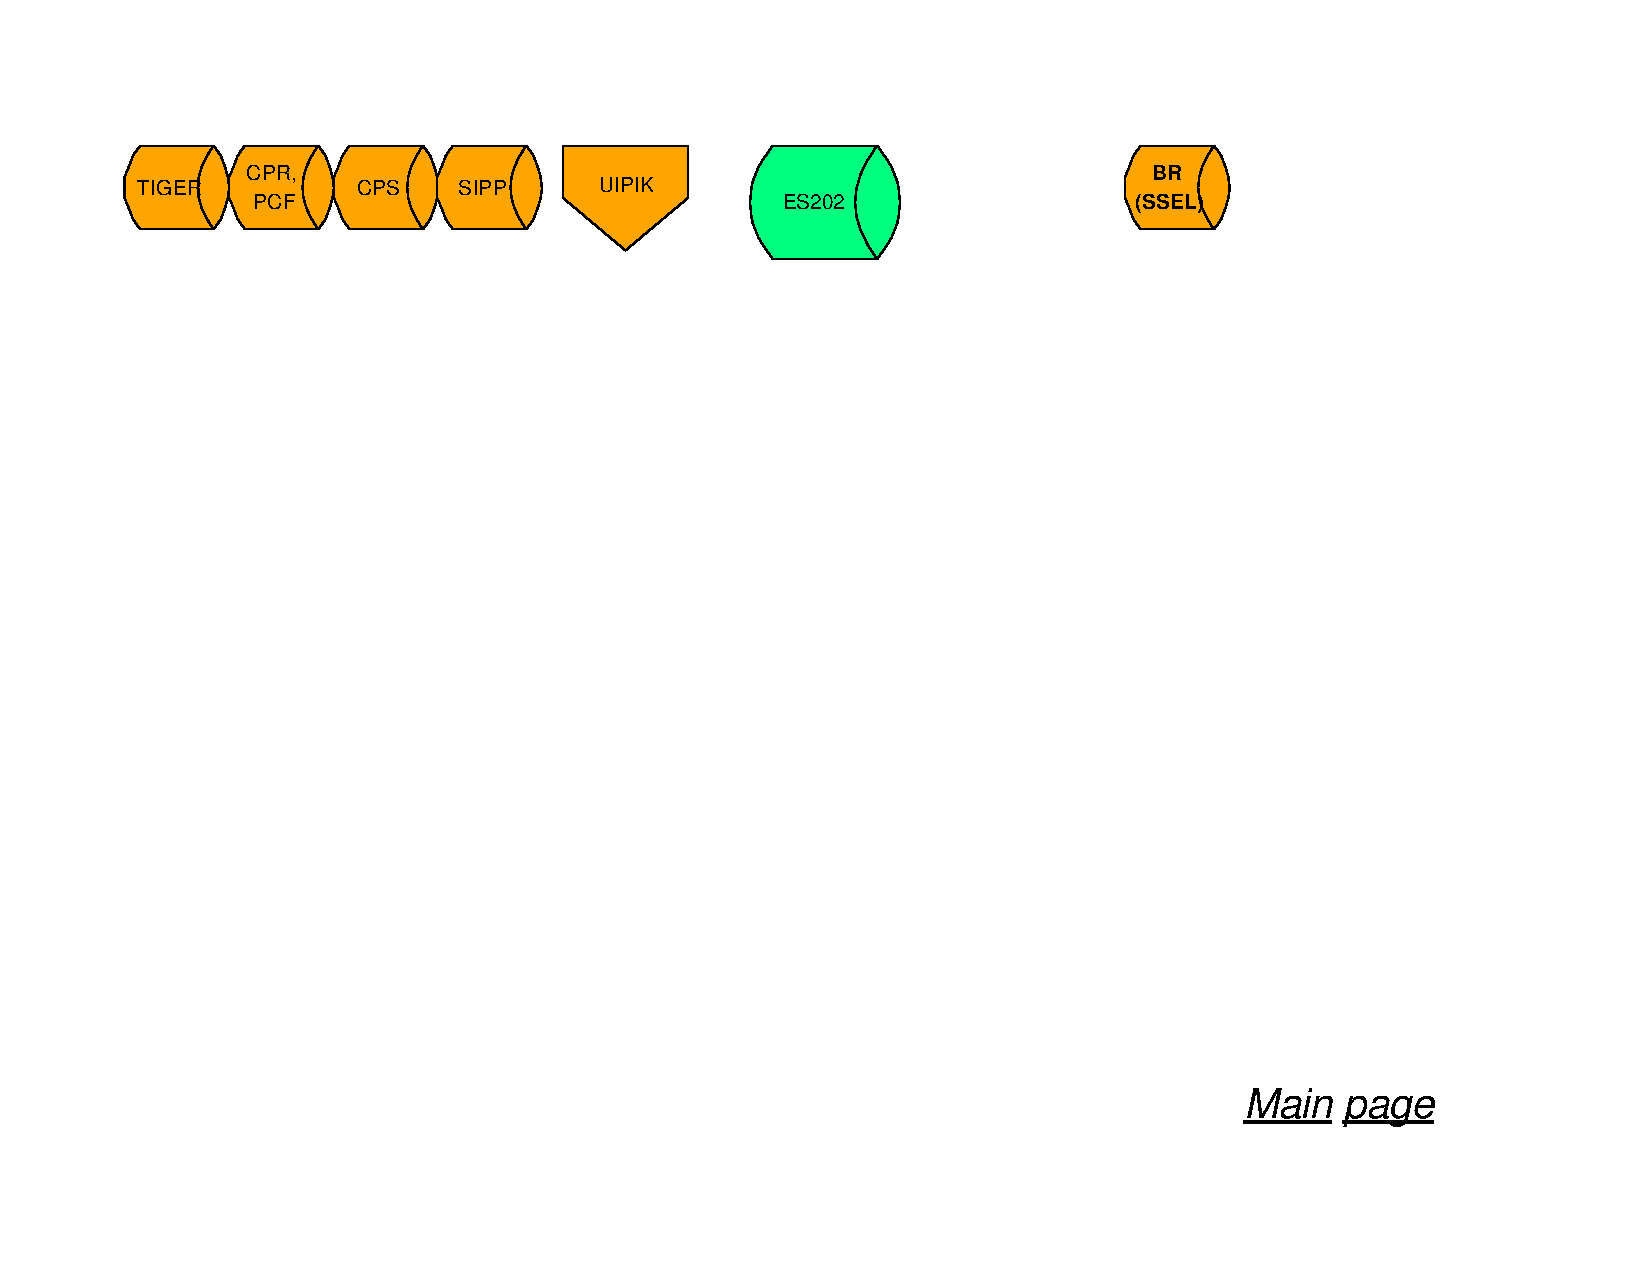
\includegraphics[scale=0.31,angle=270]{overview-data-flow/overview-data-flow-extract-stage0}}
  \onSlide*{2}{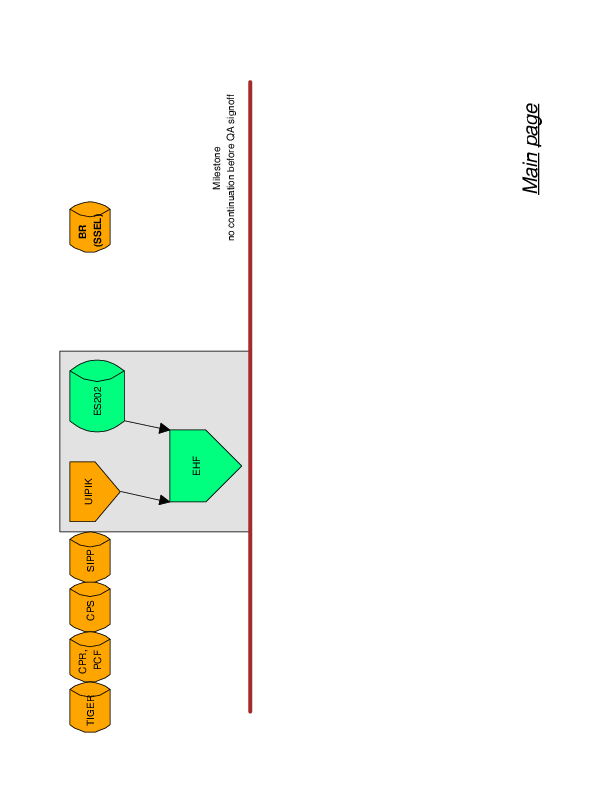
\includegraphics[scale=0.31,angle=270]{overview-data-flow/overview-data-flow-extract-stage1}}
  \onSlide*{3}{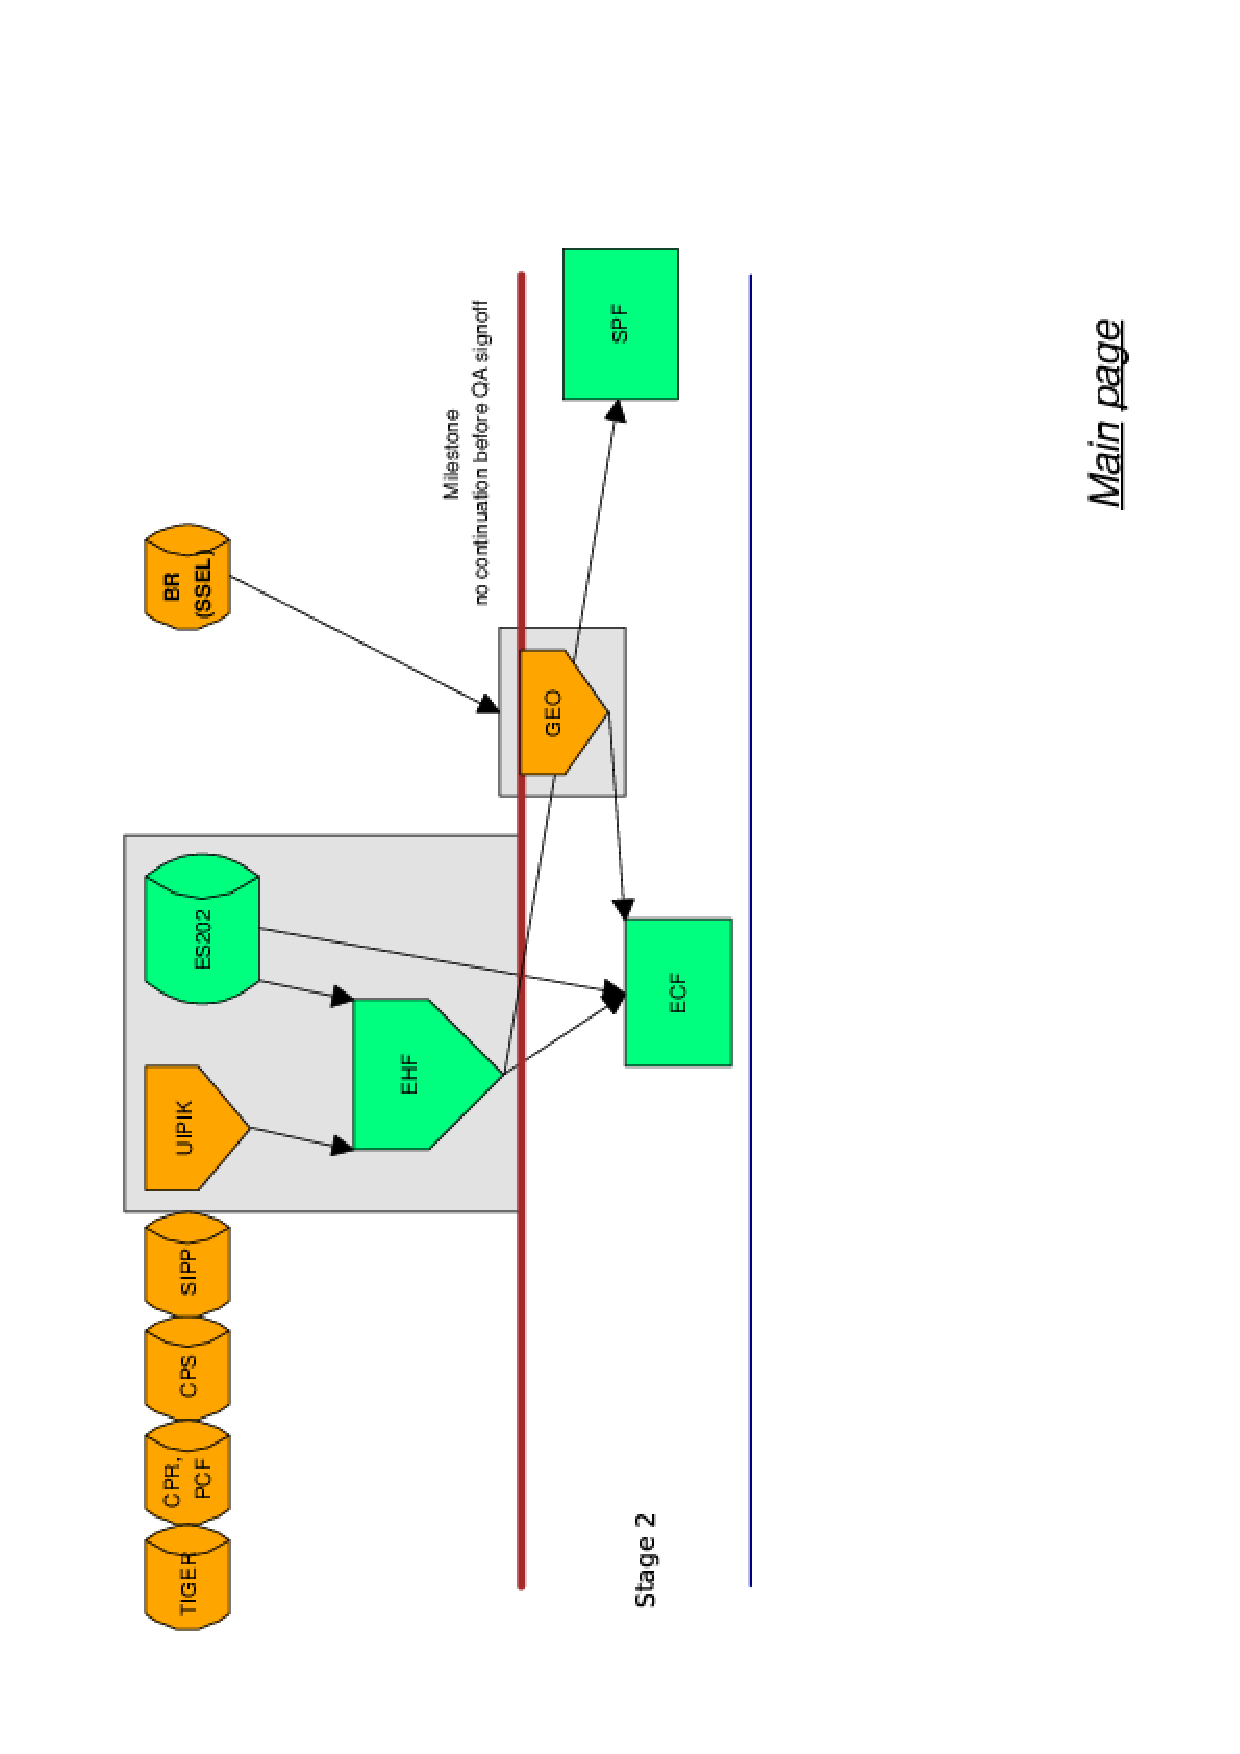
\includegraphics[scale=0.31,angle=270]{overview-data-flow/overview-data-flow-extract-stage2}}
%  \onSlide*{4}{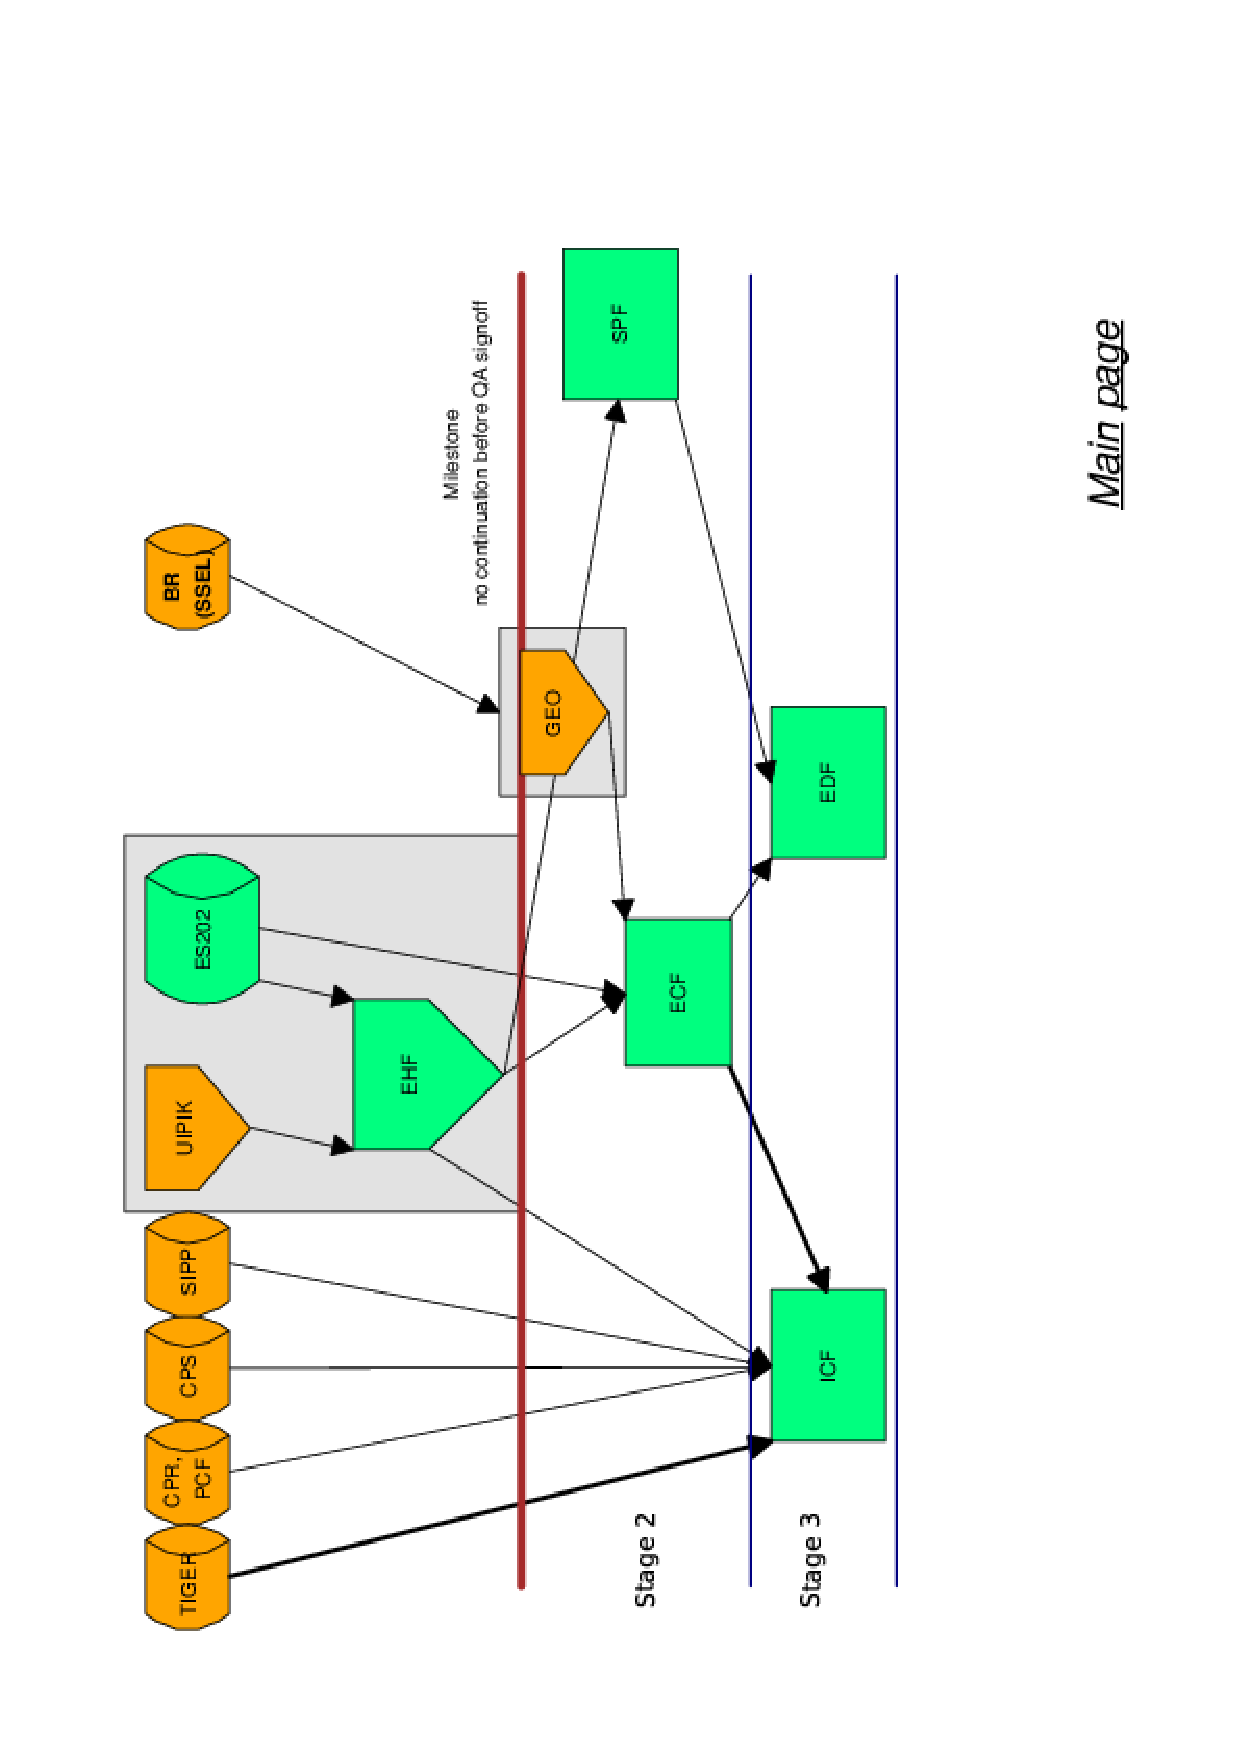
\includegraphics[scale=0.31,angle=270]{overview-data-flow/overview-data-flow-extract-stage3}}
%  \onSlide*{5}{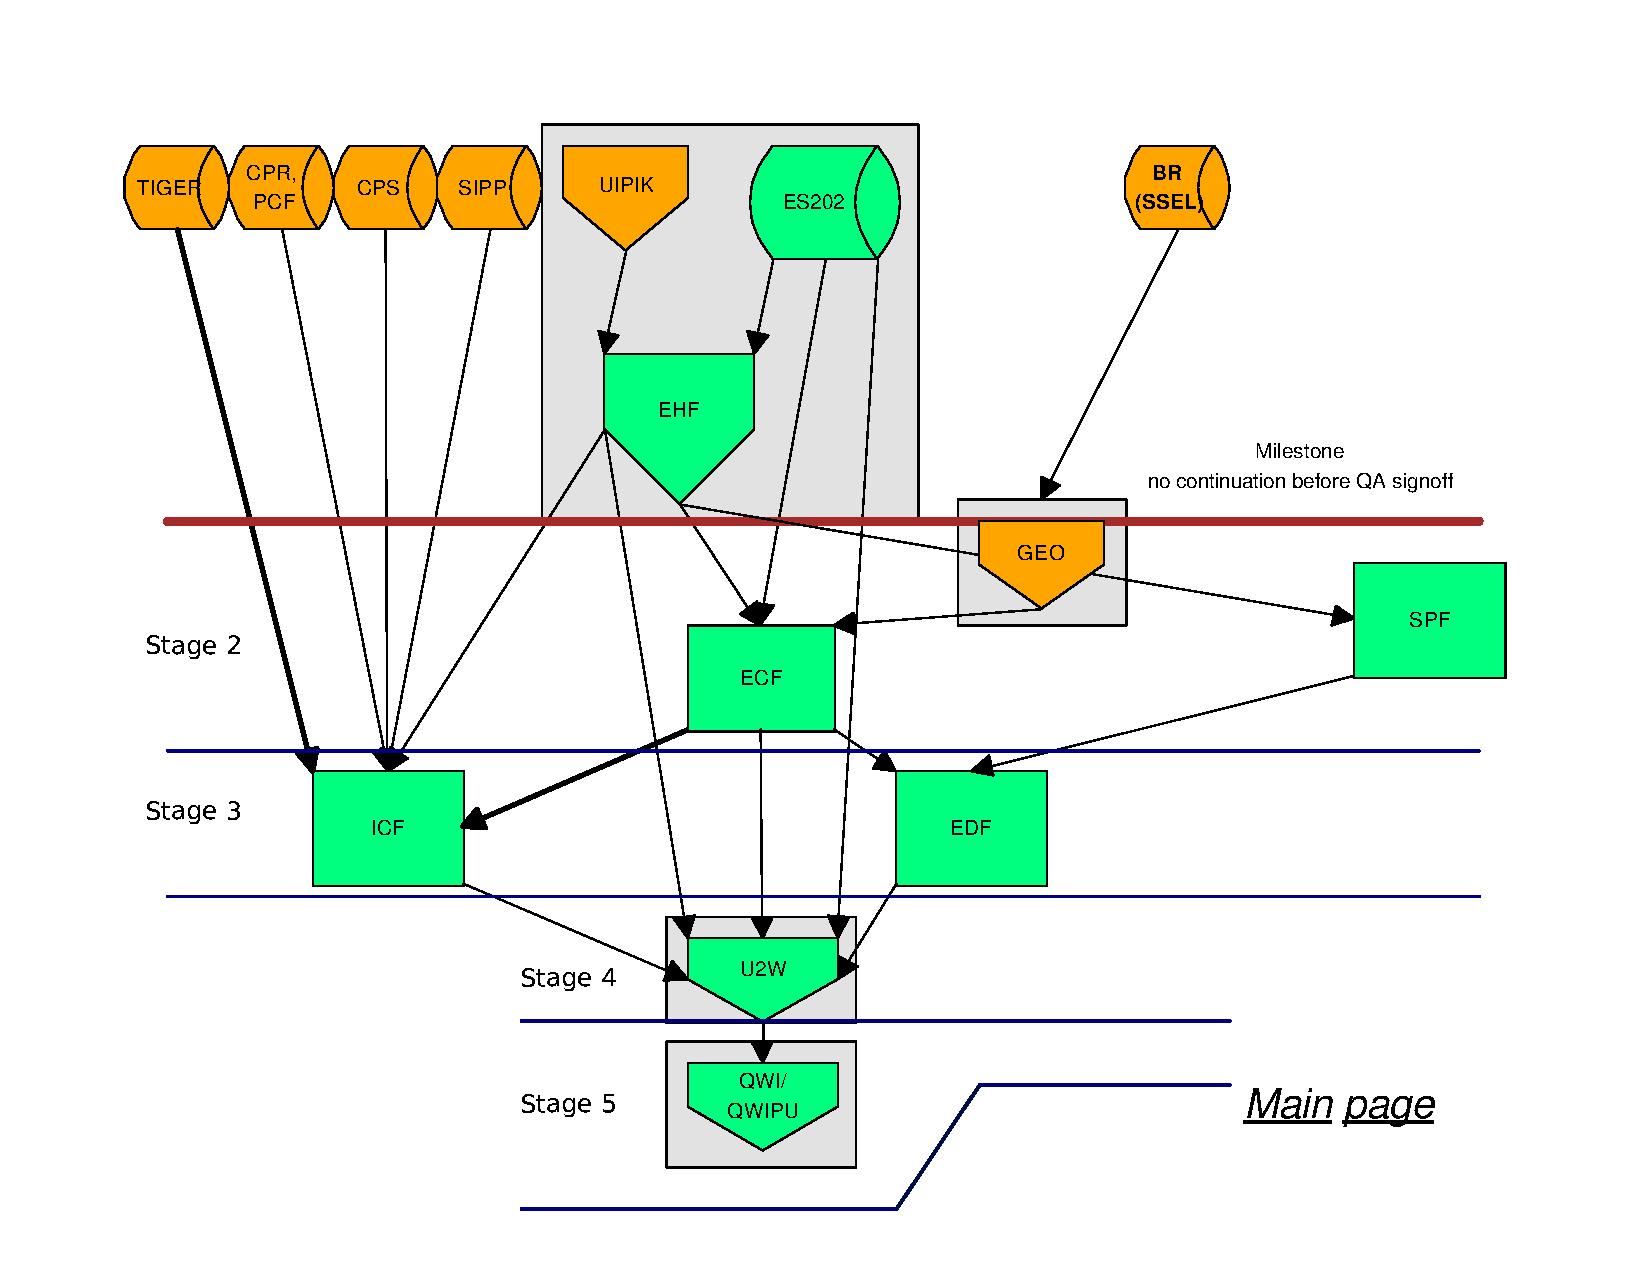
\includegraphics[scale=0.31,angle=270]{overview-data-flow/overview-data-flow-extract-qwi}}
%  \onSlide*{6}{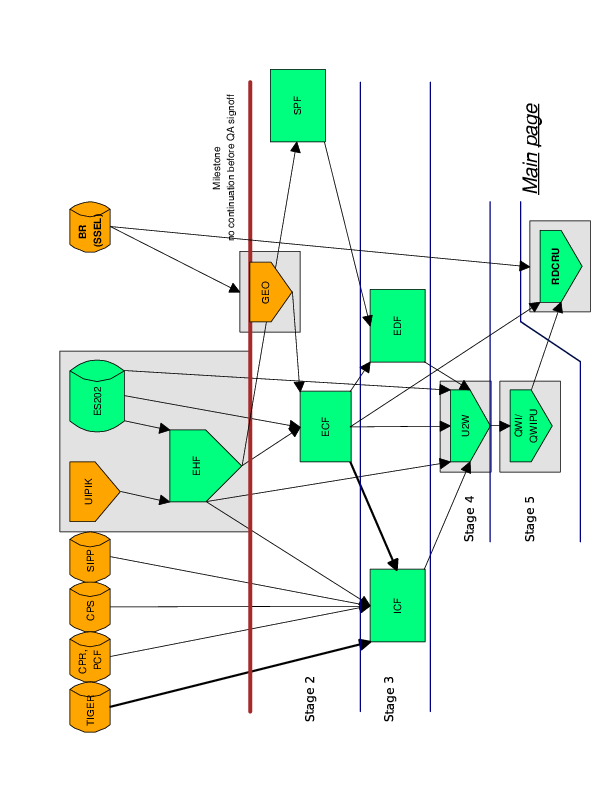
\includegraphics[scale=0.31,angle=270]{overview-data-flow/overview-data-flow-final}}
  \end{slide}
}

% ==================================================================================
% Slide 
\tsectionandpart{Forming Aggregated Estimates: QWI}
% ==================================================================================

\overlays{8}{%
  \begin{slide}{Correction of spurious worker flows}
    \begin{itemstep}
      \xitem Firm identifier: \onSlide{2}{state-specific account number}
      \xitemwait
      \xitem Account numbers can  and do change:
      \begin{itemstep}
      \xitem change in legal form 
      \xitem a merger
    \end{itemstep}
    \xitem Change in \underline{firm identifier} 
    \onSlide{7}{is {\bf the} component determining 
      when a worker changes \underline{employers}}
    \xitemwait
    \xitem $\rightarrow$ non-economic change in identifier creates spurious
    flow
  \end{itemstep}
\end{slide}
}

\overlays{4}{%
  \begin{slide}{Solution: Successor-Predecessor File}
    \begin{itemstep}
      \xitem track large worker movements between SEINs
      \xitem $\rightarrow$ link entities that have different account numbes,
      but constitute the same economic entitiy
      \xitem SPF provides  a variety of link
characteristics, based on the number of workers leaving an SEIN, in both
absolute and relative terms, and the number of workers entering an SEIN,
again in absolute and relative terms. 
      \xitem QWI: if 80\% of an SEIN's workers (the predecessor) are
observed to move to a single successor, and that successor absorbs 80\% of
its employees from a single predecessor, then all flows between those two
account numbers are filtered out, and treated as if they had never existed.
\end{itemstep}
\end{slide}
}

% ==================================================================================
\overlays{11}{%
  \begin{slide}{Attaching establishment characteristics to jobs}
    \begin{itemstep}
      \xitem Goal: achieve a high level of accuracy and detail
      \xitem Problem: \onSlide{2}{no establishment identification on wage
        record}
      \xitemwait
      \xitem 30-40\% of state-wide employment in multi-establishment firms
      \xitem Solution: probability model for employment location and imputation
      \xitem Key elements are:
      \begin{enumstep}
        \xitem distance between place-of-work and place-of-residence 
        \xitem distribution of employment across establishments of multi-establishment firms.
      \end{enumstep}
      \xitem Important practical aspects:
    \begin{itemstep}
      \xitem Non-ignorable missing data imputation
      \xitem Several million imputations every quarter
    \end{itemstep}
  \end{itemstep}
\end{slide}
}

\overlays{11}{%
  \begin{slide}{U2W: Unit to Worker Impute}
    
    \begin{itemstep}
      \xitem workers $i=1,...,I$ 
      \xitem firms $j=1,...,J$ 
      \xitem active establishments at firm $j$  $R_{jt}$ 
 %    \xitem $\mathfrak{R}=\max_{j,t}R_{jt},$ and $r=1,...,\mathfrak{R}$    index establishments.
      \xitem quarter $t$ employment of establishment $r$ in firm $j$ $N_{jrt}$ 
      \xitem $y_{ijt}$  establishment at which $i$ was employed
      \xitem $\mathcal{J}_{t}$   firms active 
      \xitem $\mathcal{I}_{jt}$  individuals employed at firm $j$ 
      \xitem $\mathcal{R}_{jt}$  set of active ($N_{jrt}>0$) establishments
      \xitem $\mathcal{R}_{jt}^{i}\subset $ $\mathcal{R}_{jt}$  set of active establishments that are feasible
      for worker $i$.
      \xitem Feasibility: an establishment $r\in \mathcal{R}_{jt}^{i}$ if $N_{jrs}>0$ for every quarter $s$ that $i$ was
      employed at $j.$
\end{itemstep}
\end{slide}
}

\overlays{8}{%
  \begin{slide}{Probability Model}
    \begin{itemstep}
    \xitem[ ]     $p_{ijrt}=\Pr \left( y_{ijt}=r\right)$
    \xitem[ ]
%
\begin{equation}
p_{ijrt}=\frac{e^{\alpha _{jrt}+x_{ijrt}^{\prime }\beta }}{\sum_{s\in 
\mathcal{R}_{jt}^{i}}e^{\alpha _{jst}+x_{ijst}^{\prime }\beta }}
\nonumber %\label{u2w:p}
\end{equation}%
%
    \xitem[ ]  $\alpha _{jrt}$  establishment- and quarter-specific effect
    \xitem[ ]  $x_{ijrt}$  time-varying vector, worker and establishment
    \xitem[ ]  $\beta $  effect on  probability of being employed at a
    particular establishment
    \xitem[ ]  Currently:
    \begin{itemstep}
      \xitem $x_{ijrt}$ is linear spline in  distance between  residence
      and  establishment
      \xitem $\alpha _{jrt}$ is a hierarchical Bayesian
      model based on  $N_{jrt}$ is 
    \end{itemstep}
  \end{itemstep}
\end{slide}
}


\overlays{4}{%
  \begin{slide}{Implementation}
    \begin{itemstep}
      \xitem[ ] Using Minnesota data,
      \xitem[ ] compute posterior modal value of $\alpha_{jrt}$
      \xitem[ ] evaluate the posterior mode of $p(\beta |\alpha , x , y )$
      \xitem[ ] maximize \\


\begin{eqnarray}
\log p\left( \beta |\alpha ,x,y\right) &\varpropto &\sum_{t=1}^{T}\sum_{j\in 
\mathcal{J}_{t}}\sum_{i\in \mathcal{I}_{jt}}\sum_{r\in \mathcal{R}%
_{jt}^{i}}d_{ijrt}\nonumber\\
%
&&\left( \alpha _{jrt}+x_{ijrt}^{\prime }\beta \right . \nonumber\\
%
&&\left . -\log \left(
\sum_{s\in \mathcal{R}_{jt}^{i}}e^{\alpha _{jst}+x_{ijst}^{\prime }\beta
}\right) \right)  \nonumber %\label{u2w:log-posterior}
\end{eqnarray}%
    \end{itemstep}
  \end{slide}
}
                                
% ==================================================================================
\overlays{5}{%
  \begin{slide}{Implementation}
    \begin{itemstep}
      \xitem use  mean and variance of $\beta $  from  Minnesota data
      \xitem take 10 draws of $\beta $ from the normal approximation (at the
mode) to $p\left( \beta |\alpha ,x,y\right)$. 
      \xitem use QCEW employment counts,  compute 10 values of $\alpha_{jt}$
      \xitem The drawn values of 
$\alpha $ and $\beta $ are used to draw 10 imputed values of place of work
from  to the posterior predictive distribution%
\begin{equation}
p\left( \tilde{y}|x,y\right) =\int \int p\left( \tilde{y}|\alpha ,\beta
,x,y\right) p\left( \alpha |N\right) p\left( \beta |\alpha ,x,y\right)
d\alpha d\beta \nonumber %.  \label{u2w:post-pred}
\end{equation}
     \xitem $\rightarrow$ 10 establishment identifiers associated with a
     job spell
\end{itemstep}
\end{slide}
}

% ==================================================================================
\overlays{14}{%
  \begin{slide}{Computing the statistics}
    \begin{itemstep}
    \xitem We now have:
    \begin{itemstep}
      \xitem Jobs identified
      \xitem Jobholder's demographics \onSlide{3}{(age, gender)}
      \xitemwait
      \xitem Establishment's  characteristics
      \onSlide{5}{(geography and industry)}
      \xitemwait
    \end{itemstep}
    \xitem Now compute
    \begin{enumstep}
      \xitem For each job, the relevant variables, defined at the
      person-level (indicators)
      \xitem Aggregate (typically sum) to the establishment level
      \xitem $\rightarrow$ establishment-level statistics, available in RDC
      \xitem Attach weights to each establishment
      \xitem Attach 'fuzz' factors to each establishment
      \xitem Final aggregation to desired geography-industry-demographic
      detail
    \end{enumstep}
    \xitem Disclosure-proof
  \end{itemstep}
  \end{slide}
}
% ==================================================================================
% Slide 
\tsectionandpart{Disclosure-proofing the QWI}
% ==================================================================================
\overlays{7}{%
  \begin{slide}{Noise-infusion }
    \begin{itemstep}
      \xitem First layer:  workplace-level  aggregation
      \begin{itemstep}
        \xitem infusion of specially constructed noise:
        \xitem 
\begin{equation}
p\left( {\delta _j } \right) = \left\{ {{%
\begin{array}{*{20}c} {\mbox{ }{\left( {b - \delta } \right)} \mathord{\left/ {\vphantom {{\left( {b - \delta } \right)} {\left( {b - a} \right)^2}}} \right. \kern-\nulldelimiterspace} {\left( {b - a} \right)^2},\;\delta \in \mbox{ 
}\left[ {a,b} \right]} \\ {{\left( {b + \delta - 2} \right)} \mathord{\left/ {\vphantom {{\left( {b + \delta - 2} \right)} {\left( {b - a} \right)^2}}} \right. \kern-\nulldelimiterspace} {\left( {b - a} \right)^2},\;\delta \in \left[ {2 - b,2 - a} \right]\mbox{ }} \\ \end{array} 
}} \right.
\end{equation}
        \xitem Result:  random noise factor
        centered around 1 with distortion of at least $a-1$ and at most $b-1$.
      \end{itemstep}
      \xitem Important properties:
      \begin{enumstep}
        \xitem for a given workplace, distortion is always
        distorted in the same direction (increased or decreased) by the same
        percentage amount in every period. 
        \xitem when  estimates are aggregated, the effects of the distortion cancel out for the vast
        majority of the estimates.
      \end{enumstep}
    \end{itemstep}
  \end{slide}
}  

\overlays{7}{%
  \begin{slide}{Item suppression}
    \begin{itemstep}
      \xitem Second layer: after aggregations
      \begin{itemstep}
        \xitem Some estimates are based on fewer than three persons or
        firms. 
        \xitem $\rightarrow$ suppression of these estimates
        \xitem Some of the estimates are based on noisy data
        \xitem $\rightarrow$  flagged as ``substantially  distorted''
      \end{itemstep}
    \end{itemstep}
  \end{slide}
}

\begin{notes}
  Second layer      of confidentiality protection occurs after the
workplace-level measures are aggregated to the higher levels. The data from many individuals and businesses are combined
into a (relatively) few estimates. This aggregation helps to conceal the
exact information about any of the individuals or businesses that underlie
the estimate.
\end{notes}

% ==================================================================================
% Slide 
\tsectionandpart{Publicly available files}
% ==================================================================================
\overlays{8}{%
  \begin{slide}{Publicly available files}
    \begin{itemstep}
      \xitem Published QWI
      \xitem[ ] $\rightarrow$ http://lehd.dsd.census.gov
      \xitem RDC
      \begin{itemstep}
        \xitem Employer characteristics files ECF $\rightarrow$ LEHD-ECF
        \xitem Establishment level flow files - Firm-level QWI
        $\rightarrow$ LEHD-QWI
        \xitem LEHD Business Register Bridge (LEHD-BRB)
        \xitem Human Capital files LEHD-HCF
    \end{itemstep}
    \xitem[ ] $\rightarrow$ http://www.ces.census.gov
  \end{itemstep}
\end{slide}
}
% ==================================================================================
% Slide 
\tsectionandpart{Conclusion}
% ==================================================================================
\overlays{4}{%
  \begin{slide}{Flow so far}
%  \onSlide*{1}{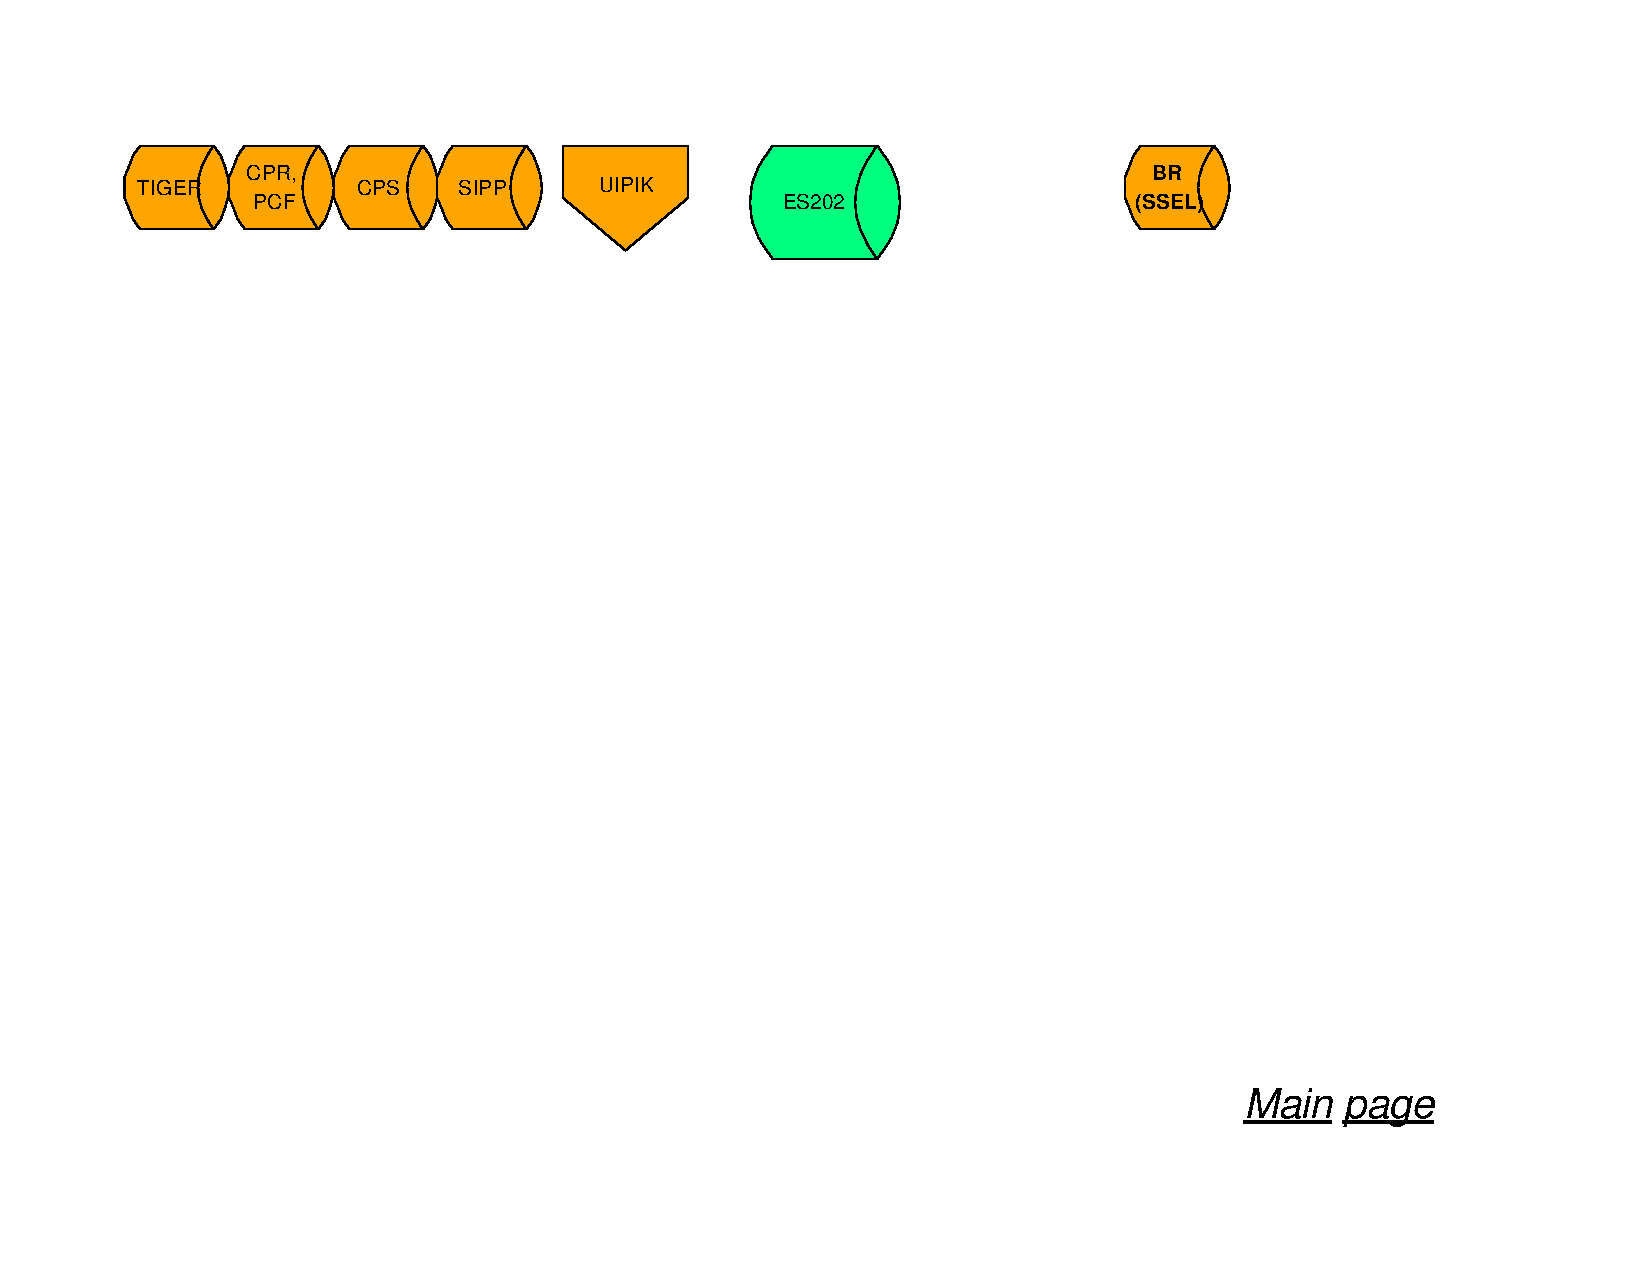
\includegraphics[scale=0.31,angle=270]{overview-data-flow/overview-data-flow-extract-stage0}}
%  \onSlide*{2}{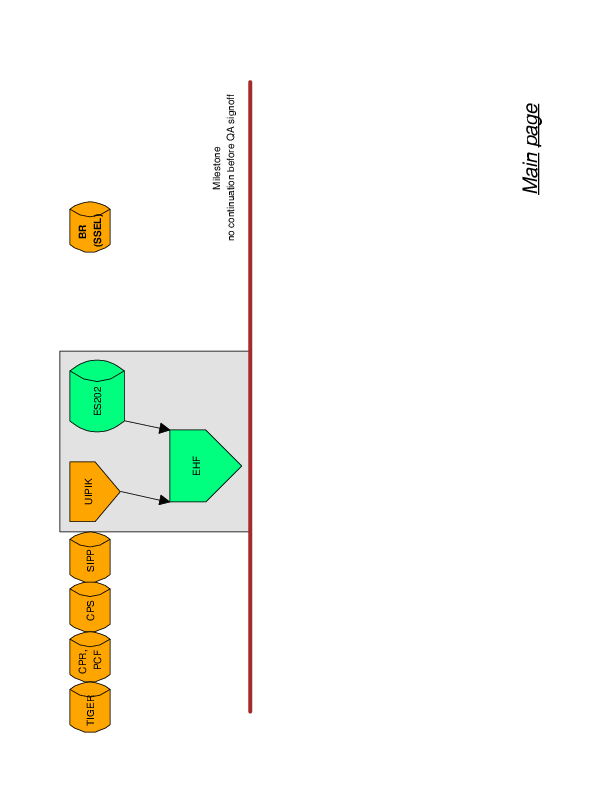
\includegraphics[scale=0.31,angle=270]{overview-data-flow/overview-data-flow-extract-stage1}}
  \onSlide*{1}{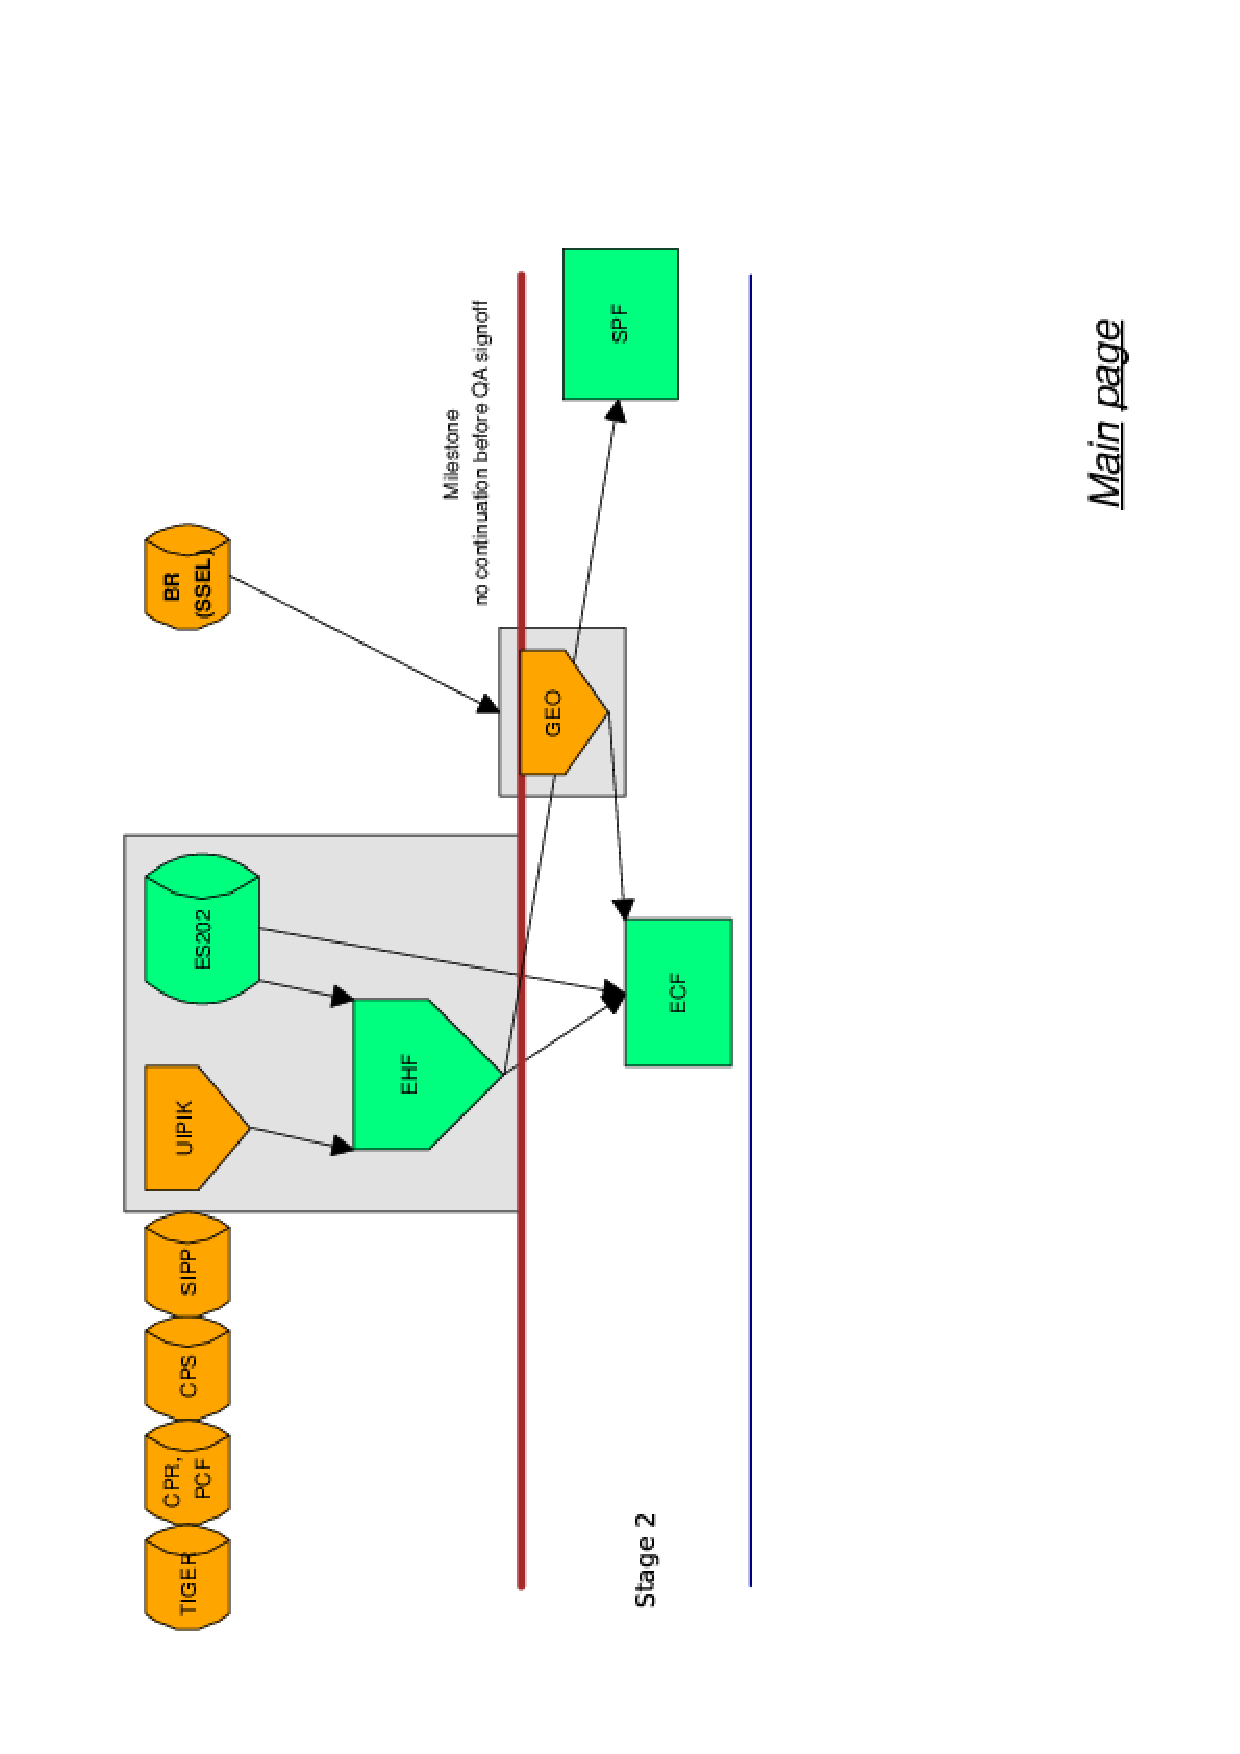
\includegraphics[scale=0.31,angle=270]{overview-data-flow/overview-data-flow-extract-stage2}}
  \onSlide*{2}{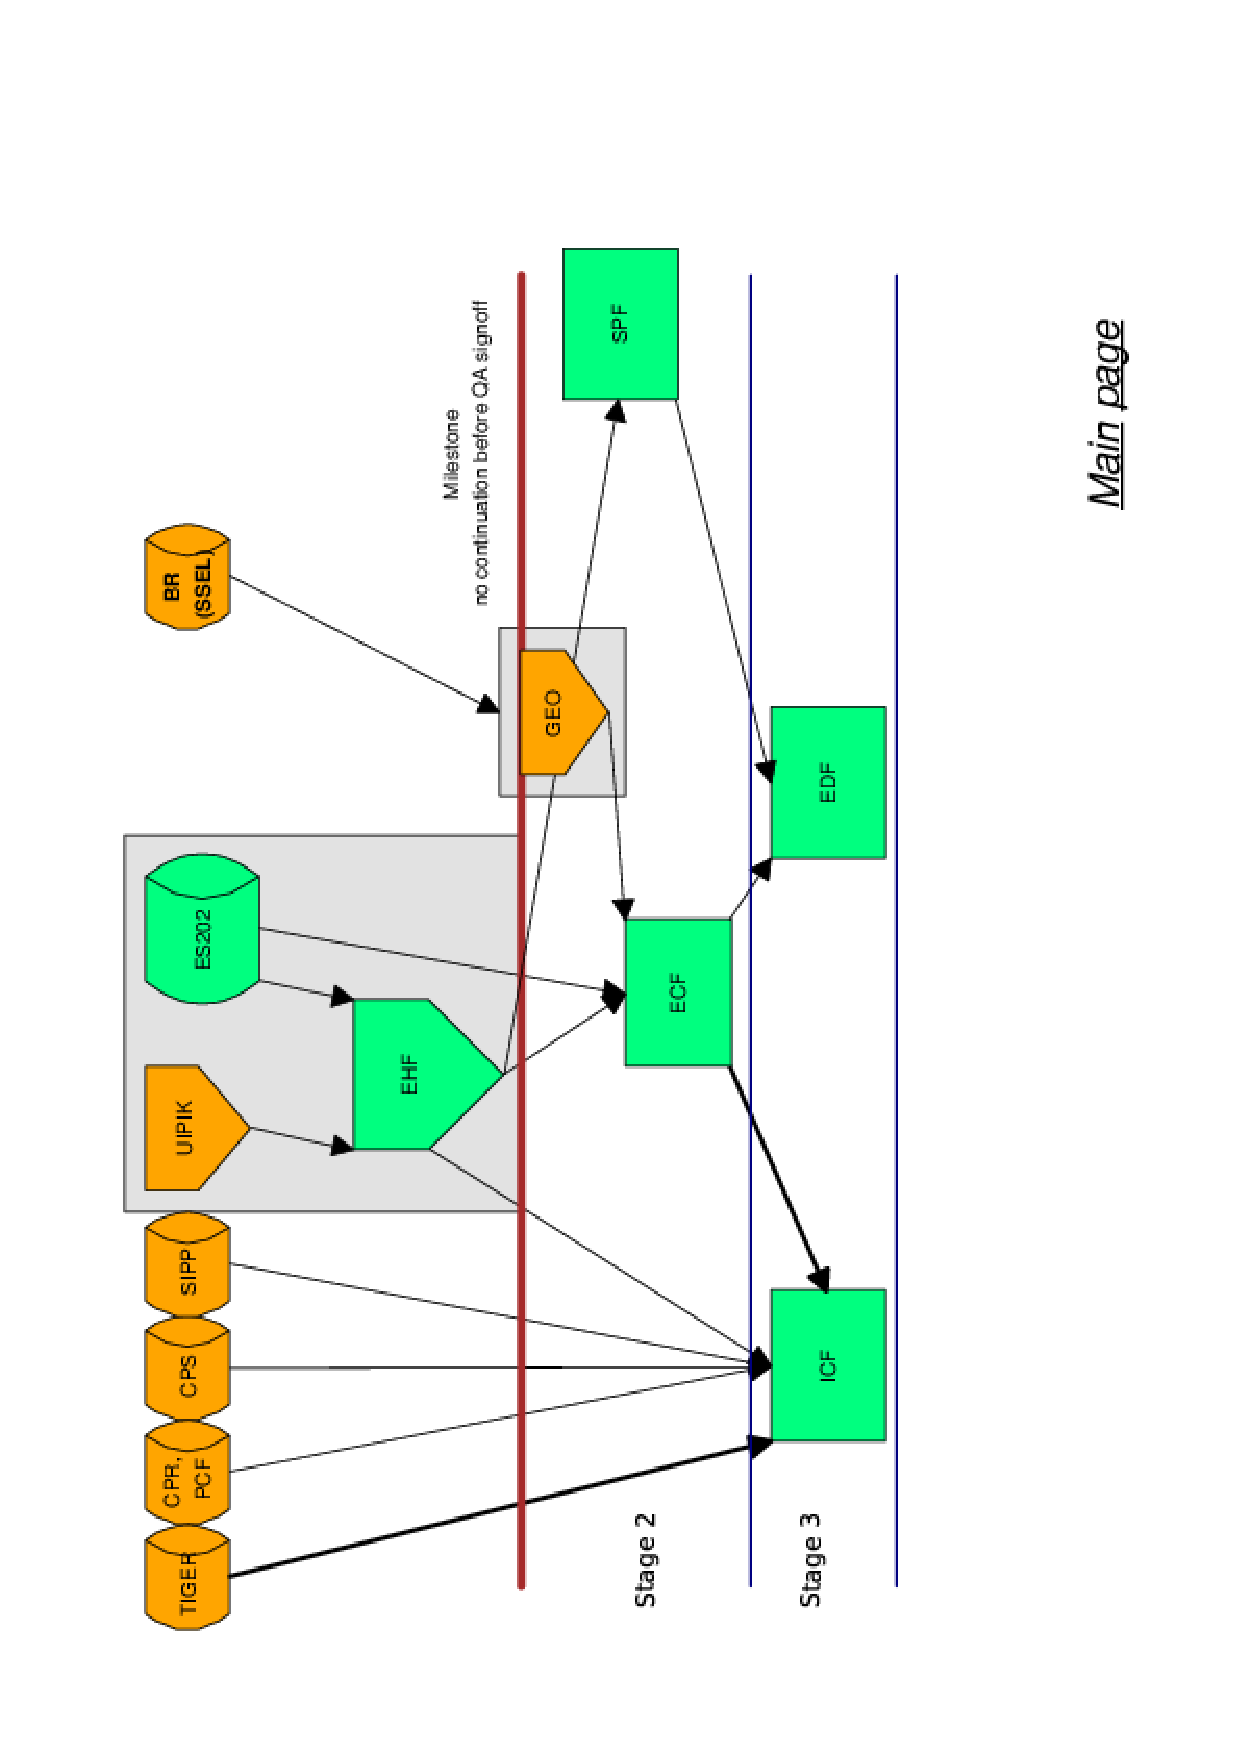
\includegraphics[scale=0.31,angle=270]{overview-data-flow/overview-data-flow-extract-stage3}}
  \onSlide*{3}{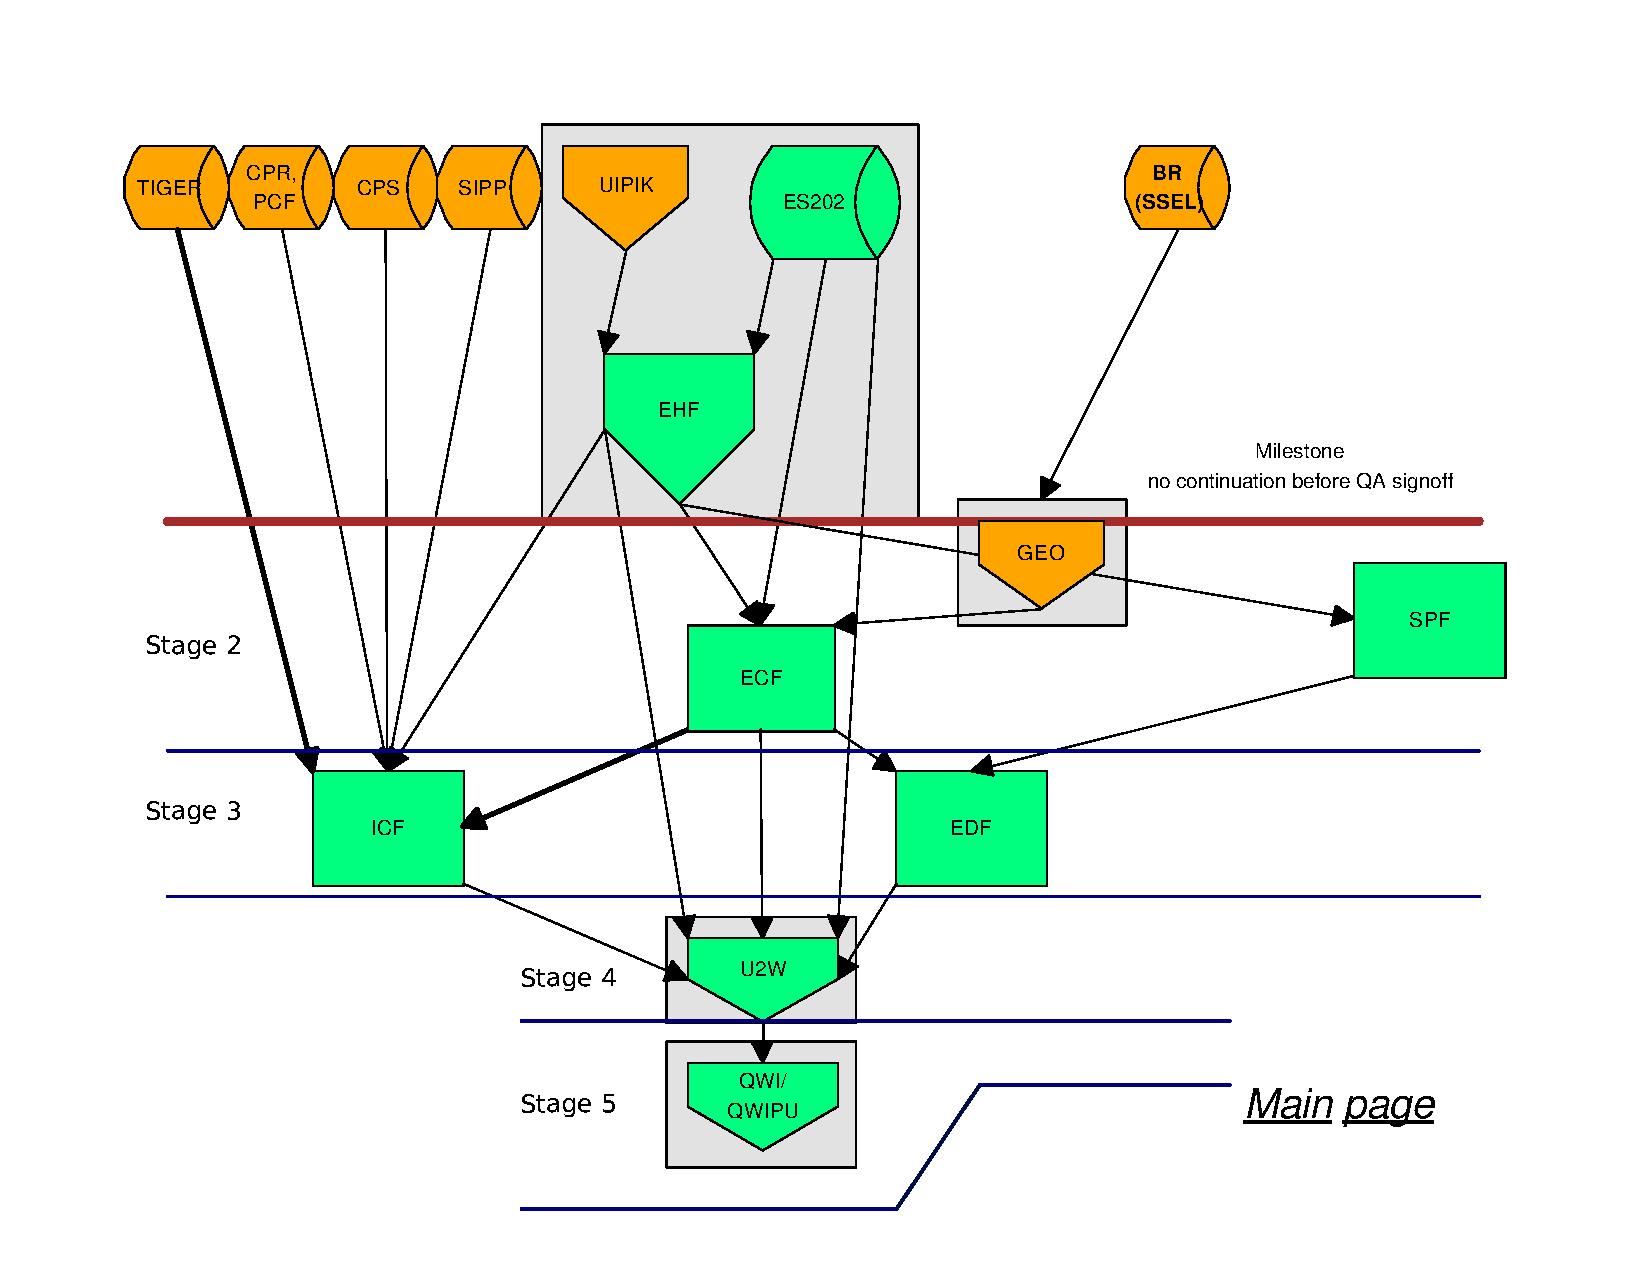
\includegraphics[scale=0.31,angle=270]{overview-data-flow/overview-data-flow-extract-qwi}}
  \onSlide*{4}{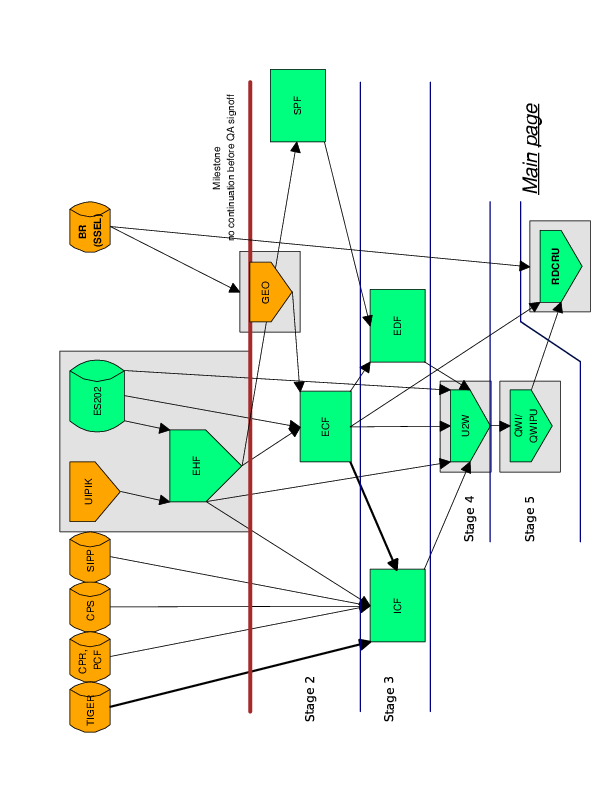
\includegraphics[scale=0.31,angle=270]{overview-data-flow/overview-data-flow-final}}
  \end{slide}
}


% ==================================================================================
% Slide 
% \overlays{2}{
% \begin{slide}{Welcome}
% \begin{itemstep}
%   \xitem Welcome to the introduction of the HA-prosper package.
%   \xitem Features of HA-prosper are:
%   \begin{itemize}
%     \xitem table of contents;
%     \xitem portrait slides support;
%     \xitem notes;
%     \xitem dual slides;
%     \xitem prosper bug solutions;
%     \xitem and lots more.
%   \end{itemize}
% \end{itemstep}
% \end{slide}
% }
% % ==================================================================================
% 
% 
% % ==================================================================================
% % Slide 4
% \overlays{2}{
% \begin{slide}{Styles}
% \begin{itemstep}
%   \xitem The HA-prosper packages adds functionality to prosper, but\dots
%   \xitem The available styles show how to extend these possibilities
%    even further and for instance:
%   \begin{itemize}
%     \xitem embed additional navigational elements on slides;
%     \xitem use multiple slide layouts in the same presentation;
%     \xitem etcetera.
%   \end{itemize}
% \end{itemstep}
% \end{slide}
% }
% % ==================================================================================
% 
% 
% % ==================================================================================
% % Slide 5
% \tsectionandpart{Features}
% % ==================================================================================
% 
% 
% % ==================================================================================
% % Slide 6
% \overlays{4}{
% \begin{slide}{Table of contents}
% \begin{itemstep}
%   \xitem A table of contents can be put on every slide;
%   \xitem A table of contents entry is created from the slide title
%    or from text that is given as an optional argument;
%   \xitem The table of contents has the following features:
%   \begin{itemize}
%     \xitem Highlighting of the current slide or section is possible;
%     \xitem Items can be omitted;
%     \xitem Parts of the table of contents can be hidden when these are
%      unnecessary.
%   \end{itemize}
%   \xitem The style that you use should of course support the inclusion
%    of the table of contents.
% \end{itemstep}
% \end{slide}
% }
% % ==================================================================================
% 
% 
% % ==================================================================================
% % Slide 7
% \overlays{6}{
% \begin{slide}{More features}
% HA-prosper contains more features which are fully described in the manual.
% \begin{itemstep}[sstart=2]
%   \xitem Portrait slides;
%   \xitem Notes;
%   \xitem Dual slides;
%   \xitem Blackslide;
%   \xitem and a lot more\dots
% \end{itemstep}
% \end{slide}
% }
% % ==================================================================================
% 
% 
% % ==================================================================================
% % Slide 8
% \overlays{5}{
% \begin{slide}{Prosper bug solutions}
% \begin{itemstep}
%   \xitem Numbering of equations, tables and figures on overlays is supported be default;
%   \xitem Custom counters can be protected throughout the presentation;
%   \xitem The `\textbackslash and' command for authors is supported;
%   \xitem Improved placement of left and right footers;
%   \xitem and more.
% \end{itemstep}
% \end{slide}
% }
% % ==================================================================================
% 
% 
% % ==================================================================================
% % Slide 9
% \tsectionandpart{Contributions and questions}
% % ==================================================================================
% 
% 
% % ==================================================================================
% % Slide 10
% \overlays{3}{
% \begin{slide}{Contributions}
% \begin{itemstep}
%   \xitem Contributions are always welcome.
%   \xitem In case you want to contribute a style, which offers undocumented
%    features, please insert both
%   \begin{itemize}
%     \xitem documentation;
%     \xitem an example that demonstrates all the features that your style provides.
%   \end{itemize}
%   \xitem You can contact
%     \href{http://stuwww.uvt.nl/~hendri/Personal/contact.html}{\underline{Hendri Adriaens}}
%     (click the link) in case you have comments or questions about
%     developing a new template or if want to submit your style.
% \end{itemstep}
% \end{slide}
% }
% % ==================================================================================
% 
% 
% % ==================================================================================
% % Slide 11
% \overlays{2}{
% \begin{slide}{Questions}
% \begin{itemstep}
%   \xitem If you have questions, please first consult the documentation
%    of the following packages (depending on your problem):
%   \begin{itemize}
%     \xitem HA-prosper;
%     \xitem Prosper;
%     \xitem Hyperref;
%     \xitem PSTricks.
%   \end{itemize}
%   \xitem In case you cannot find the answer and your question is related
%    to HA-prosper, you can post a message to the HA-prosper mailinglist:\par
%   \href{http://listserv.surfnet.nl/archives/ha-prosper.html}{http://listserv.surfnet.nl/archives/ha-prosper.html}.
% \end{itemstep}
% \end{slide}
% }
% ==================================================================================


\end{document}
